\documentclass[tikz,border=2pt]{standalone}
\usepackage{newtxtext,newtxmath}
\usetikzlibrary{arrows.meta,positioning}
\definecolor{bear}{HTML}{1F4E8C}\definecolor{bearL}{HTML}{DCE6F2}
\definecolor{apx}{HTML}{B8741A}\definecolor{apxL}{HTML}{F6E3C3}
\definecolor{bad}{HTML}{C8462D}\definecolor{g1}{HTML}{555555}\definecolor{g4}{HTML}{EDEDED}\definecolor{txt2}{HTML}{6B6B6B}
\begin{document}
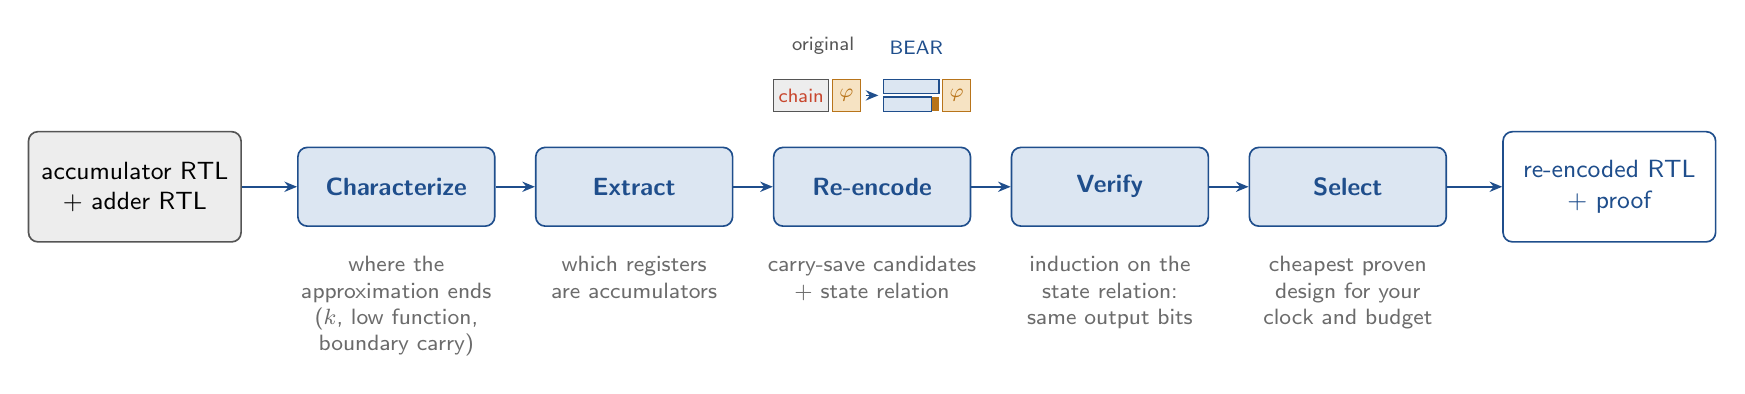
\begin{tikzpicture}[x=1mm,y=1mm,>={Stealth[length=1.6mm,width=1.3mm]},font=\sffamily\small,
  stage/.style={draw=bear,fill=bearL,rounded corners=1.2mm,line width=0.6pt,minimum width=25mm,minimum height=10mm,align=center,text=bear},
  io/.style={draw=g1,fill=g4,rounded corners=1.2mm,line width=0.6pt,minimum width=27mm,minimum height=14mm,align=center},
  note/.style={font=\sffamily\footnotesize,text=txt2,align=center}]
\node[io] (in) at (0,0) {accumulator RTL\\+ adder RTL};
\node[stage,right=7mm of in] (c) {\textbf{Characterize}};
\node[stage,right=5mm of c] (e) {\textbf{Extract}};
\node[stage,right=5mm of e] (r) {\textbf{Re-encode}};
\node[stage,right=5mm of r] (v) {\textbf{Verify}};
\node[stage,right=5mm of v] (s) {\textbf{Select}};
\node[io,right=7mm of s,draw=bear,fill=white,text=bear] (out) {re-encoded RTL\\+ proof};
\foreach \a/\b in {in/c,c/e,e/r,r/v,v/s,s/out} \draw[->,line width=0.8pt,bear] (\a) -- (\b);
\node[note,below=2.5mm of c] {where the\\approximation ends\\($k$, low function,\\boundary carry)};
\node[note,below=2.5mm of e] {which registers\\are accumulators};
\node[note,below=2.5mm of r] {carry-save candidates\\+ state relation};
\node[note,below=2.5mm of v] {induction on the\\state relation:\\same output bits};
\node[note,below=2.5mm of s] {cheapest proven\\design for your\\clock and budget};
% 示意：原环与 BEAR 环
\begin{scope}[shift={(r.north)},yshift=4mm]
  \node[font=\sffamily\scriptsize,text=g1,anchor=south east] at (-1,6.5) {original};
  \draw[g1,fill=g4,line width=0.4pt] (-12.5,0.5) rectangle (-5.5,4.5); \node[font=\sffamily\scriptsize,text=bad] at (-9,2.5) {chain};
  \draw[apx,fill=apxL,line width=0.4pt] (-5.0,0.5) rectangle (-1.5,4.5); \node[font=\sffamily\scriptsize,text=apx] at (-3.25,2.5) {$\varphi$};
  \draw[->,bear,line width=0.6pt] (-0.8,2.5) -- (0.8,2.5);
  \node[font=\sffamily\scriptsize,text=bear,anchor=south west] at (1,6.5) {BEAR};
  \draw[bear,fill=bearL,line width=0.4pt] (1.5,2.7) rectangle (8.5,4.5); \draw[bear,fill=bearL,line width=0.4pt] (1.5,0.5) rectangle (7.6,2.3);
  \fill[apx] (7.6,0.5) rectangle (8.5,2.3);
  \draw[apx,fill=apxL,line width=0.4pt] (9.0,0.5) rectangle (12.5,4.5); \node[font=\sffamily\scriptsize,text=apx] at (10.75,2.5) {$\varphi$};
\end{scope}
\end{tikzpicture}
\end{document}
